%------------------------------------------------------------------------
% Grafiken
%\usepackage{pstricks-add}
\usepackage{tikz}
\usepackage{tikz-qtree}
\usepackage{circuitikz}
%\usepackage{tikz-uml}
\ctikzset{voltage/distance from node=.5}% in \pgf@circ@Rlen units 
\ctikzset{voltage/distance from line=.25}% pos. between 0 and 1 
\ctikzset{voltage/bump b/.initial=1.5}% 
 
%\usepackage{trfsigns}
 
\usepackage{pgfplots}
\pgfplotsset{compat=newest}
\usetikzlibrary{plotmarks,math,positioning,shapes,arrows,backgrounds,circuits.logic.IEC,circuits.ee.IEC,decorations.pathmorphing,patterns,shapes.geometric,calc,fit,matrix}

%% NUR unter Windows mit texlive notwendig
\makeatletter
\global\let\tikz@ensure@dollar@catcode=\relax

\newcommand{\symbolbegr}{
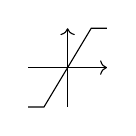
\begin{tikzpicture}
	\draw[black] (0,0)--(0.2,0)--(0.8,1)--(1,1);
	\draw[black,->] (0,0.5)--(1,0.5);
	\draw[black,->] (0.5,0)--(0.5,1);
\end{tikzpicture}
}

\newcommand{\symbolhyst}{
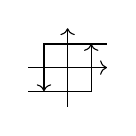
\begin{tikzpicture}
	\draw[black,->] (0,0.2)--(0.8,0.2)--(0.8,0.8);
	\draw[black,<-] (0.2,0.2)--(0.2,0.8)--(1,0.8);
	
	\draw[black,->] (0,0.5)--(1,0.5);
	\draw[black,->] (0.5,0)--(0.5,1);
\end{tikzpicture}
}

\pgfdeclarepatternformonly{north east lines wide}%
   {\pgfqpoint{-1pt}{-1pt}}%
   {\pgfqpoint{10pt}{10pt}}%
   {\pgfqpoint{9pt}{9pt}}%
   {
     \pgfsetlinewidth{0.4pt}
     \pgfpathmoveto{\pgfqpoint{0pt}{0pt}}
     \pgfpathlineto{\pgfqpoint{9.1pt}{9.1pt}}
     \pgfusepath{stroke}
    }

\pgfdeclarepatternformonly{north west lines wide}%
   {\pgfqpoint{-1pt}{-1pt}}%
   {\pgfqpoint{10pt}{10pt}}%
   {\pgfqpoint{9pt}{9pt}}%
   {
     \pgfsetlinewidth{0.4pt}
     \pgfpathmoveto{\pgfqpoint{0pt}{9.1pt}}
     \pgfpathlineto{\pgfqpoint{9.1pt}{0pt}}
     \pgfusepath{stroke}
    }

\pgfkeys{/pgf/.cd,
  parallelepiped offset x/.initial=2mm,
  parallelepiped offset y/.initial=2mm
}
\pgfdeclareshape{parallelepiped}
{
  \inheritsavedanchors[from=rectangle] % this is nearly a rectangle
  \inheritanchorborder[from=rectangle]
  \inheritanchor[from=rectangle]{north}
  \inheritanchor[from=rectangle]{north west}
  \inheritanchor[from=rectangle]{north east}
  \inheritanchor[from=rectangle]{center}
  \inheritanchor[from=rectangle]{west}
  \inheritanchor[from=rectangle]{east}
  \inheritanchor[from=rectangle]{mid}
  \inheritanchor[from=rectangle]{mid west}
  \inheritanchor[from=rectangle]{mid east}
  \inheritanchor[from=rectangle]{base}
  \inheritanchor[from=rectangle]{base west}
  \inheritanchor[from=rectangle]{base east}
  \inheritanchor[from=rectangle]{south}
  \inheritanchor[from=rectangle]{south west}
  \inheritanchor[from=rectangle]{south east}
  \backgroundpath{
    % store lower right in xa/ya and upper right in xb/yb
    \southwest \pgf@xa=\pgf@x \pgf@ya=\pgf@y
    \northeast \pgf@xb=\pgf@x \pgf@yb=\pgf@y
    \pgfmathsetlength\pgfutil@tempdima{\pgfkeysvalueof{/pgf/parallelepiped offset x}}
    \pgfmathsetlength\pgfutil@tempdimb{\pgfkeysvalueof{/pgf/parallelepiped offset y}}
    \def\ppd@offset{\pgfpoint{\pgfutil@tempdima}{\pgfutil@tempdimb}}
    \pgfpathmoveto{\pgfqpoint{\pgf@xa}{\pgf@ya}}
    \pgfpathlineto{\pgfqpoint{\pgf@xb}{\pgf@ya}}
    \pgfpathlineto{\pgfqpoint{\pgf@xb}{\pgf@yb}}
    \pgfpathlineto{\pgfqpoint{\pgf@xa}{\pgf@yb}}
    \pgfpathclose
    \pgfpathmoveto{\pgfqpoint{\pgf@xb}{\pgf@ya}}
    \pgfpathlineto{\pgfpointadd{\pgfpoint{\pgf@xb}{\pgf@ya}}{\ppd@offset}}
    \pgfpathlineto{\pgfpointadd{\pgfpoint{\pgf@xb}{\pgf@yb}}{\ppd@offset}}
    \pgfpathlineto{\pgfpointadd{\pgfpoint{\pgf@xa}{\pgf@yb}}{\ppd@offset}}
    \pgfpathlineto{\pgfqpoint{\pgf@xa}{\pgf@yb}}
    \pgfpathmoveto{\pgfqpoint{\pgf@xb}{\pgf@yb}}
    \pgfpathlineto{\pgfpointadd{\pgfpoint{\pgf@xb}{\pgf@yb}}{\ppd@offset}}
  }
}

\pgfdeclareshape{zohswitch}{
  \inheritsavedanchors[from=rectangle]
  \inheritanchorborder[from=rectangle]
  \inheritanchor[from=rectangle]{center}
  \inheritanchor[from=rectangle]{base}
  \inheritanchor[from=rectangle]{north}
  \inheritanchor[from=rectangle]{north east}
  \inheritanchor[from=rectangle]{east}
  \inheritanchor[from=rectangle]{south east}
  \inheritanchor[from=rectangle]{south}
  \inheritanchor[from=rectangle]{south west}
  \inheritanchor[from=rectangle]{west}
  \inheritanchor[from=rectangle]{north west}
  \behindbackgroundpath{
    %  store lower right in xa/ya and upper right in xb/yb
    \southwest \pgf@xa=\pgf@x \pgf@ya=\pgf@y
    \northeast \pgf@xb=\pgf@x \pgf@yb=\pgf@y
    
    \pgfpathmoveto{\pgfpoint{\pgf@xa}{(\pgf@ya + \pgf@yb)/2}}
    %\pgfpathlineto{\pgfpoint{(\pgf@xa + \pgf@xb)/4}{(\pgf@ya + \pgf@yb)/2}}
    \pgfpathlineto{\pgfpoint{\pgf@xb}{\pgf@yb}}
    %\pgfpathmoveto{\pgfpoint{\pgf@xa + \pgf@xb)* 3 / 4 }{(\pgf@ya + \pgf@yb)/2}}
    %\pgfpathlineto{\pgfpoint{\pgf@xb}{(\pgf@ya + \pgf@yb)/2}}
    
    \pgfsetlinewidth{.15mm}\pgfsetarrows{-}\pgfsetstrokecolor{black}\pgfusepath{stroke}
 }
}

\pgfdeclareshape{datastore}{
  \inheritsavedanchors[from=rectangle]
  \inheritanchorborder[from=rectangle]
  \inheritanchor[from=rectangle]{center}
  \inheritanchor[from=rectangle]{base}
  \inheritanchor[from=rectangle]{north}
  \inheritanchor[from=rectangle]{north east}
  \inheritanchor[from=rectangle]{east}
  \inheritanchor[from=rectangle]{south east}
  \inheritanchor[from=rectangle]{south}
  \inheritanchor[from=rectangle]{south west}
  \inheritanchor[from=rectangle]{west}
  \inheritanchor[from=rectangle]{north west}
%  \behindbackgroundpath{
    %  store lower right in xa/ya and upper right in xb/yb
%    \southwest \pgf@xa=\pgf@x \pgf@ya=\pgf@y
%    \northeast \pgf@xb=\pgf@x \pgf@yb=\pgf@y
%    \pgfpathmoveto{\pgfpoint{\pgf@xa}{\pgf@ya}}
%    \pgfpathlineto{\pgfpoint{\pgf@xb}{\pgf@ya}}
%    \pgfpathmoveto{\pgfpoint{\pgf@xa}{\pgf@yb}}
%    \pgfpathlineto{\pgfpoint{\pgf@xb}{\pgf@yb}}

    % Draw it, always black, arrowless and .5mm width
%    \pgfsetlinewidth{.5mm}\pgfsetarrows{-}\pgfsetstrokecolor{black}\pgfusepath{stroke}
% }
  \backgroundpath{
    %  store lower right in xa/ya and upper right in xb/yb
    \southwest \pgf@xa=\pgf@x \pgf@ya=\pgf@y
    \northeast \pgf@xb=\pgf@x \pgf@yb=\pgf@y
    \pgfpathmoveto{\pgfpoint{\pgf@xa}{\pgf@ya}}
    \pgfpathlineto{\pgfpoint{\pgf@xb}{\pgf@ya}}
    \pgfpathmoveto{\pgfpoint{\pgf@xa}{\pgf@yb}}
    \pgfpathlineto{\pgfpoint{\pgf@xb}{\pgf@yb}}
 }
}

% coilup, coildown decorations
% code by Hans-Peter E. Kristiansen
% in http://tex.stackexchange.com/a/43605/3954
% Parameters: \pgfdecorationsegmentamplitude, \pgfdecorationsegmentlength,

\pgfdeclaredecoration{coilup}{coil}
{
  \state{coil}[switch if less than=%
    1.5\pgfdecorationsegmentlength+%
    \pgfdecorationsegmentaspect\pgfdecorationsegmentamplitude+%
    \pgfdecorationsegmentaspect\pgfdecorationsegmentamplitude to last,
               width=+\pgfdecorationsegmentlength]
  {
    \pgfpathcurveto
    {\pgfpoint@oncoil{0    }{ 0.555}{1}}
    {\pgfpoint@oncoil{0.445}{ 1    }{2}}
    {\pgfpoint@oncoil{1    }{ 1    }{3}}
    \pgfpathmoveto{\pgfpoint@oncoil{1    }{-1    }{9}}
    \pgfpathcurveto
    {\pgfpoint@oncoil{0.445}{-1    }{10}}
    {\pgfpoint@oncoil{0    }{-0.555}{11}}
    {\pgfpoint@oncoil{0    }{ 0    }{12}}
  }
  \state{last}[width=.5\pgfdecorationsegmentlength+%
    \pgfdecorationsegmentaspect\pgfdecorationsegmentamplitude+%
    \pgfdecorationsegmentaspect\pgfdecorationsegmentamplitude,next state=final]
  {
    \pgfpathcurveto
    {\pgfpoint@oncoil{0    }{ 0.555}{1}}
    {\pgfpoint@oncoil{0.445}{ 1    }{2}}
    {\pgfpoint@oncoil{1    }{ 1    }{3}}
    \pgfpathmoveto{\pgfpoint@oncoil{2    }{ 0    }{6}}
  }
  \state{final}
  {
  \pgfpathmoveto{\pgfpointdecoratedpathlast}
  }
}


% coildown decoration
%
% Parameters: \pgfdecorationsegmentamplitude, \pgfdecorationsegmentlength,

\pgfdeclaredecoration{coildown}{coil}
{
  \state{coil}[switch if less than=%
    1.5\pgfdecorationsegmentlength+%
    \pgfdecorationsegmentaspect\pgfdecorationsegmentamplitude+%
    \pgfdecorationsegmentaspect\pgfdecorationsegmentamplitude to last,
               width=+\pgfdecorationsegmentlength]
  {
    \pgfpathmoveto{\pgfpoint@oncoil{1    }{1    }{3}}
    \pgfpathcurveto
    {\pgfpoint@oncoil{1.555}{ 1    }{4}}
    {\pgfpoint@oncoil{2    }{ 0.555}{5}}
    {\pgfpoint@oncoil{2    }{ 0    }{6}}
    \pgfpathcurveto
    {\pgfpoint@oncoil{2    }{-0.555}{7}}
    {\pgfpoint@oncoil{1.555}{-1    }{8}}
    {\pgfpoint@oncoil{1    }{-1    }{9}}
  }
  \state{last}[width=.5\pgfdecorationsegmentlength+%
    \pgfdecorationsegmentaspect\pgfdecorationsegmentamplitude+%
    \pgfdecorationsegmentaspect\pgfdecorationsegmentamplitude,next state=final]
  {
    \pgfpathmoveto{\pgfpoint@oncoil{1    }{ 1    }{3}}
    \pgfpathcurveto
    {\pgfpoint@oncoil{1.555}{ 1    }{4}}
    {\pgfpoint@oncoil{2    }{ 0.555}{5}}
    {\pgfpoint@oncoil{2    }{ 0    }{6}}
  }
  \state{final}
  {
  \pgfpathlineto{\pgfpointdecoratedpathlast}
  }
}

\def\pgfpoint@oncoil#1#2#3{%
  \pgf@x=#1\pgfdecorationsegmentamplitude%
  \pgf@x=\pgfdecorationsegmentaspect\pgf@x%
  \pgf@y=#2\pgfdecorationsegmentamplitude%
  \pgf@xa=0.083333333333\pgfdecorationsegmentlength%
  \advance\pgf@x by#3\pgf@xa%
}

\makeatother
\usetikzlibrary{trees}

% Dataflows
\tikzstyle{prozess} = [draw, thick, rounded corners, inner sep=.3cm]
\tikzstyle{function} = [draw, thick, circle]
\tikzstyle{ifunction} = [draw, thick, circle split,minimum size=30mm, font=\small]
\tikzstyle{datastore} = [draw, very thick, shape=datastore, inner sep=.3cm]
\tikzstyle{to} = [->, >=stealth', shorten >=1pt, semithick, font=\sffamily\footnotesize]
\tikzstyle{dto} = [->, dashed, >=stealth', shorten >=1pt, semithick, font=\sffamily\footnotesize]
\tikzstyle{wto} = [-, color=white, >=stealth', shorten >=1pt, semithick, font=\sffamily\footnotesize]
\tikzstyle{bto} = [<->, >=stealth', shorten >=1pt, semithick, font=\sffamily\footnotesize]
\tikzstyle{ccircle} = [path picture={ \draw[black] (path picture bounding box.south east) -- (path picture bounding box.north west) (path picture bounding box.south west) -- (path picture bounding box.north east);}]

% Controlflows
\tikzstyle{block} = [draw, fill=white, rectangle, minimum height=3em, minimum width=4em]
\tikzstyle{rblock} = [draw, fill=white, circle, inner sep=0pt,minimum size=1mm]
\tikzstyle{wobblock} = [fill=white, rectangle, minimum height=3em, minimum width=5em]
\tikzstyle{nlblock} = [draw, postaction={draw,line width=0.25mm,white}, line width=0.5mm, black, fill=white, rectangle, minimum height=3em, minimum width=5em]
%\tikzstyle{sum} = [draw,circle]
\tikzstyle{branch} = [circle,inner sep=0pt,minimum size=1mm,fill=black,draw=black]
\tikzstyle{nvbranch} = [circle,inner sep=0pt,minimum size=1mm,fill=white,draw=white, fill opacity=0, draw opacity=0]
\tikzstyle{vecBranch} = [circle,inner sep=0pt,minimum size=2mm,fill=black,draw=black]
\tikzstyle{input} = [coordinate]
\tikzstyle{output} = [coordinate] 
\tikzstyle{coord} = [coordinate] 
\tikzstyle{pinstyle} = [pin edge={to-,thin,black}] 
\tikzstyle{vecArrow} = [thick, decoration={markings,mark=at position
   1 with {\arrow[semithick]{open triangle 60}}},
   double distance=1.4pt, shorten >= 5.5pt,
   preaction = {decorate},
   postaction = {draw,line width=1.4pt, white,shorten >= 4.5pt}]
\tikzstyle{vecWithoutArrow} = [thick,
   double distance=1.4pt,
   postaction = {draw,line width=1.4pt, white}]
\tikzset{
  Pfeil/.style={thick,shorten >=#1,shorten <=#1,->,>=latex}, % für Peile
  UPfeil/.style={black,Pfeil=#1,font={\sffamily\itshape}},% für Spannungspfeile
  IPfeil/.style={black,Pfeil=#1,font={\ttfamily\itshape}} % für Strompfeile
}   
\tikzstyle{box}=[rectangle, draw, thick]

\tikzstyle{sum} = [draw, fill=black, circle, node distance=0.5cm, inner sep=0pt,minimum size=0.5em]

\tikzstyle{sumGraph} = [draw, circle, node distance=1cm, fill=black, minimum size=0.5em]

\tikzstyle{circ} = [draw, circle, node distance=1cm]